\newpage
\chapter{Managing with radiative effects}
\label{sect:rad_eff}

\mbox{}\vspace{-\baselineskip}


For the simulation of the radiative effects the procedure described in Chapter~7 of the report~\cite{twopeg} was used. However, the task of combining this procedure with the simulation of the target motion is not straightforward. The following two methods were therefore developed and tested.


\section{ Naive method}

In this approach the simulation of the radiative effects was done first, while the simulation of the target motion is performed after that, using the radiated values of $\widetilde{W}$ and $\widetilde{Q^2}$ as well as radiated four-momenta of the incoming and scattered electrons as a starting point.

%The usual free proton TWOPEG version of the event generator can also work in 

This method is implemented into the free proton TWOPEG (which also has a complementary moving target mode) and executed under the options $F_{fermi}=1$ and $F_{rad}=1$~or~2.

\section{Advanced method}

In this approach the simulation of the radiative effects is merged with that of the target motion in the following way\footnote[1]{Eqs.~(7.2) to (7.5) are given in the report~\cite{twopeg}.}.


\begin{itemize}

\item The Fermi momentum is generated and the true value of the final hadron system invariant mass $W_{true}$ is calculated according to Eq.~\eqref{w_fermi_nonsm}.

\item The nonradiated cross section in Eqs.~(7.2) to (7.5) are taken for the true value $W_{true}$. To combine transverse and longitudinal structure functions into the full virtual photoproduction cross section and to convert it then to the electroproduction one, the values of $\varepsilon_{T}$, $\varepsilon_{L}$, and $\Gamma_{v}$ were calculated in the quasi-Lab frame.

%\item The factor $R_{radsoft}$ in Eq.~(7.2) as well as the quantities $\rho_{ini}$ and $\rho_{fin}$ in the integrals given by Eq.(7.3) and Eq.(7.4), respectively, are assumed to be calculated in the Lab frame. The grid over the radiated photon energy and the maximal allowed energy of the radiated photon ($\omega_{max}^{ini}$ and $\omega_{max}^{fin}$) in these integrals is also defined in the Lab frame.

\item The factor $R_{radsoft}$ in Eq.~(7.2) as well as the integrals given by Eqs.~(7.3) and (7.4) are calculated in the Lab frame. 

\item The maximal allowed energy of the radiated photon ($\omega_{max}^{ini}$ and $\omega_{max}^{fin}$ given by Eqs.~(7.3) and (7.4)) is restricted by the demand to produce a pion pair. This restriction is imposed in the quasi-Lab frame, although the values of $\omega_{max}^{ini}$ and $\omega_{max}^{fin}$ are calculated in the Lab system.


%In the integrals given by Eq.(7.3) and Eq.(7.3) $\omega_{max}^{ini}$ and $\omega_{max}^{fin}$ are also calculated in the Lab frame, but  the condition of achievement of the double pion production threshold is imposed in the quasi-Lab frame.
\end{itemize}


This method is implemented into the TWOPEG-D version of the event generator, which always works in the moving target mode ($F_{fermi}=1$).

These two methods turned out to give almost indistinguishable missing mass and momentum distributions and very similar weighted $W$ distributions.
Nevertheless, the second approach is thought to be the preferential one and, therefore, is recommended. 

% results with regards to the cross-section propagation as well as missing mass and momentum distributions.
%Although this two methods turned out to give almost identical results, the second one is treated as the preferential one.


\begin{figure}[!ht]
\begin{center}
\framebox{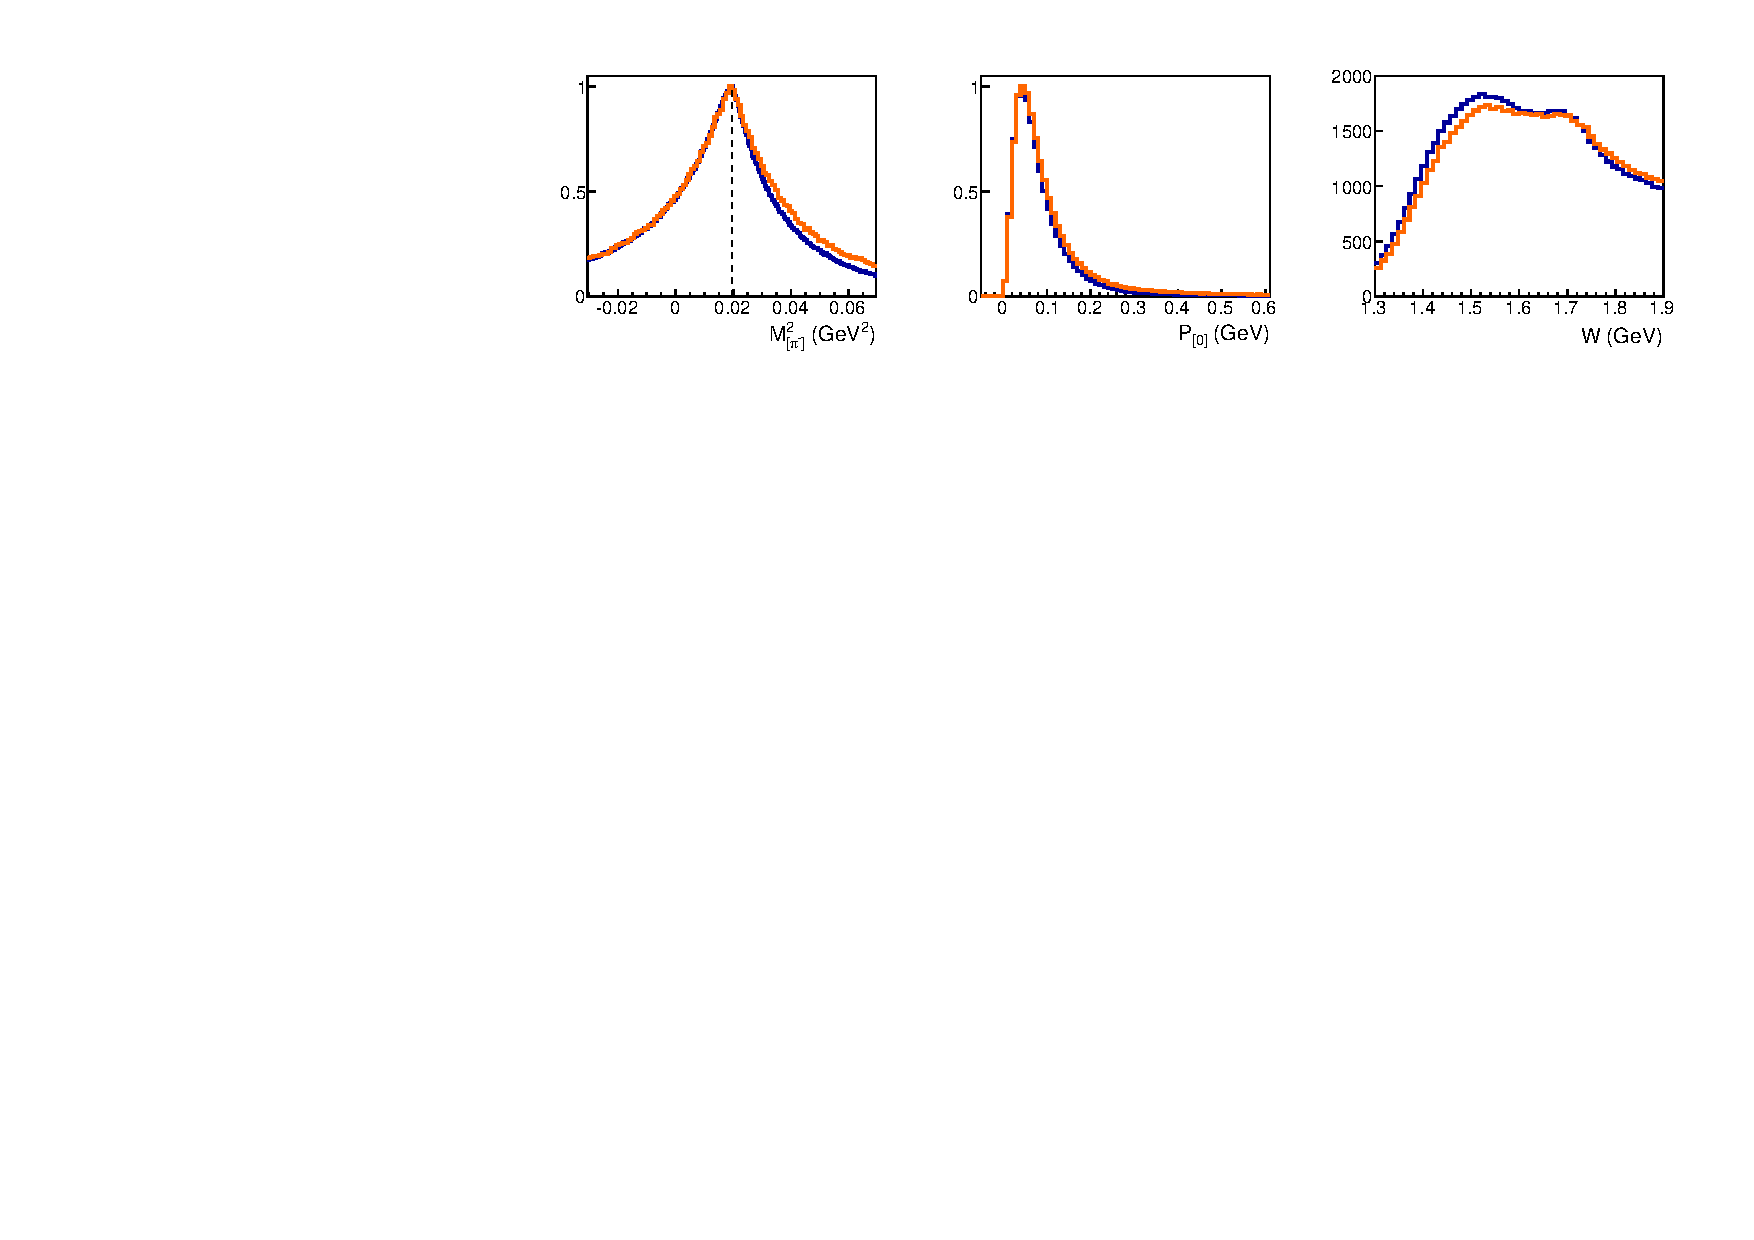
\includegraphics[width=16cm]{pictures/w_ferm_rad_norad_comp.pdf}}
\end{center}
\caption{\small  The comparison of the event distributions produced by TWOPEG-D with radiative effects (orange curves) and without (blue curves). The left and middle plots correspond to the quantities $M_{[\pi^{-}]}^{2}$ and $P_{[0]}$, respectively, which were calculated according to Eqs.~\eqref{eq:quant_targ_at_rest}. The right plot shows the comparison of the weighted $W_{sm}$ distributions. The example is given for $E_{beam} = 2$~GeV, 1.3~GeV $< W_{sm} <$ 1.9~GeV, and 0.4~GeV$^2$ $< Q^{2}<$ 0.5~GeV$^2$.  }
\label{fig:w_ferm_rad_norad_comp}
\end{figure}

Figure~\ref{fig:w_ferm_rad_norad_comp} shows the comparison of the event distributions produced by TWOPEG-D with radiative effects (orange curves) and without (blue curves). The left and middle plots correspond to the quantities $M_{[\pi^{-}]}^{2}$ and $P_{[0]}$, respectively, which are given by Eqs.~\eqref{eq:quant_targ_at_rest}. These  quantities were calculated assuming (like in experiment) that $P_{e}^{Lab}$ and $P_{e'}^{Lab}$ are not affected by the radiative effects, while $P_{p'}^{Lab}$, $P_{\pi^{+}}^{Lab}$, and $P_{\pi^{-}}^{Lab}$, on the contrary, take them into account. The right plot shows the comparison of the weighted $W_{sm}$ distributions. 

%Although for the simulation of the radiative effects TWOPEG-D uses exactly the same procedure as that described in Chapter~(7) of the report~\cite{twopeg}, the need to combine it properly with the simulation of the target motion effects has brought us to additional complications.


%goal of combining this procedure with the technique of the simulating the motion of the target proton turned out to be rather complicated.
